\chapter{Aktuelle Engine-Entwicklung}
\label{chap:engine-uebersicht}

%% Zitat:
% https://twitter.com/CompSciFact/status/527816734863265792
\epigraph{"`Even if your code was perfect when you released it, it still needs to be maintained because the world around it is changing."'}{Unbekannt}

Spiele- und Grafikengines sind inzwischen äußerst komplexe Softwareprojekte. Zu den Anfangszeiten der Spieleentwicklung konnten Spiele von Einzelpersonen oder sehr kleinen Teams entwickelt werden. Gegenwärtig sind Gesamtteamstärken von über 100 Kernentwicklern aus unterschiedlichen Disziplinen keine Seltenheit \parencite[Kapitel 8, Abschnitt: "`The Problem with Large Teams"']{keith2010agile}.

\begin{quote}
% 
"`While Unity has a core team of around 150 engineers, and Epic has around 100 concentrating on Unreal Engine 4, Jones says it's hard for him to compare --- because while there are only around 50 engineers working directly on the engine, every Crytek project across its eight studios has its own engine R\&D team, and `every single one of those games is delivering technology back into the engine.'"'\footnote{Juni http://www.gamasutra.com/view/news/218947/What\_separates\_CryEngine\_from\_its\_competition.php}
\end{quote}

Im Vergleich: Das erste \textit{Prince of Persia} wurde in der Zeit von 1985 bis 1989 alleine von Jordan Mechner entwickelt \parencite{Mechner1993} und das erste \textit{Doom} in der Zeit von 1992 bis 1993 von John Carmack, John Romero und Dave D. Taylor \parencite{Kushner2003}.

Im letzten Jahr hat sich der Markt der kommerziellen Spiele- und Grafik-Engines sehr verändert. Neben veränderten Lizenzmodellen hat einer der wichtigsten Entwickler von kommerziellen Engines, \textit{Epic Games}, die \textit{Unreal Engine 4} der Allgemeinheit gegenüber geöffnet. Zuvor mussten noch sechsstellige Beträge für den Zugang zum Quelltext bezahlt werden. 

Inzwischen ruft \textit{Epic Games} zur direkten Mitarbeit an ihrer Engine auf. Das bringt für beide Seiten Vorteile. Zwar muss der beitragende Entwickler auf seine Rechte am Code verzichten\footnote{Abschnitt 8. 8. Feedback and Contributions: https://www.unrealengine.com/eula}, doch kann er direkten Einfluss auf die Entwicklung kommerzieller Schlüsselsoftware nehmen. Und auf der anderen Seite kann das Unternehmen den Eifer der Entwickler kommerziell verwerten und eine Gemeinschaft um die Engine aufbauen.

\section{Agile Projektstrukturen}\label{sec:engines-projektstrukturen}

Komplexe Softwareprojekte erfordern neue Projektstrukturen, und dementsprechend haben sich die Projektstrukturen aber auch die Organisationformen der Teams im Laufe der Zeit gewandelt. Mit der Professionalisierung der Branche sind auch die Anforderungen an die Software klar definiert: Das Softwareprojekt ist langfristing angelegt (Spiele-Engines auf Jahrzente), soll dementsprechend robust und flexibel, wartbar, zugänglich und angemessen verständlich sein. Projektstrukturen sind inzwischen häufig auf kurze Iterationszyklen ausgelegt. Unternehmen wie \textit{Blizzard Entertainment}\footnote{http://eu.blizzard.com/de-de/company/careers/university-relations/job-desc/new-grad/engineer-automation.html} oder \textit{CPP Games} \parencite[Kapitel 8]{keith2010agile} setzen auf agile Softwareentwicklung.

Durch die kurzen Iterationszyklen werden konkrete Ziele in Reichweite gesteckt, damit sich das Erreichen oder Nichterreichen zeitnah abschätzen lässt. Zusätzlich helfen sie den Überblick über den momentanen Aufgabenbereich zu behalten und das Ziel nicht aus den Augen zu verlieren. Weiter sollen die kurze Iterationszyklen dem Entwicklerteam ermöglichen, auf die sich verändernde Umwelt zu reagieren und sich auf neue Anforderungen flexibel einzustellen. 

% Mit zunehmender Teamgröße steigt der Kommunikationaufwand zwischen den Teammitgliedern. 
Ja nach Umsetzung der Projektorganisation, werden autonome Teams aus maximal 7-11 Personen und interdisziplinär zusammengestellt \parencite[Kapitel 8]{keith2010agile}. Die Teamgröße wird möglichst klein gehalten, da mit wachsener Teamgröße der Kommunikationsaufwand deutlich\footnotemark ansteigt.

\footnotetext{Mit der Formel $n*(n - 1)/2$, mit $n$ für die Anzahl der Teammitglieder, lässt sich die Anzahl der paarweisen Kommunikationskanäle zwischen Teammitgliedern errechen. Dies entspricht einem exponentiellen Wachstum.}

\section{Herausforderungen}\label{sec:engines-herausforderungen}

Besonders Engines unterliegen besonderen Anforderungen. Im Gegensatz zu Computerspielen, die meistens einem abgesteckten Entwicklungszyklus und Lebenszyklus unterliegen, werden Engines mit langfristigen Zielen entwickelt. Da Engines, wie \textit{Unity} oder die \textit{Unreal Engine}, als Framework das Rückrat für viele unterschiedliche Spiele bilden, sollten sie robust aber auch flexibel, erweiterbar und wartbar sein. Dies sind klassische nichtfunktionale Anforderungen an Softwareprojekte, die sich nicht direkt messen lassen.

Die technischen Anforderungen in der Spielebranche verändern sich durch die kurzen Hardware-Lebenszyklen jährlich, insbesondere im PC und mobilen Sektor. Hinzu kommt, dass die Branche starken Trends unterworfen ist; heute noch gefragte Genres können morgen durch ein anderes an den Rand gedrängt werden. Dies erhöht zusätzlich die Anforderungen an die Wart- und Erweiterbarkeit.

In der Softwareentwicklung, in der mehrere kleinere Teams auf einer gemeinsamen Codebasis arbeiten, ist der Quelltext Hauptkommunikationmittel unter den Softwareentwicklern. Die Form der Zusammenarbeit und die Produktivität bestimmt sich aus der Architektur der Software und umgekehrt bestimmt die Form der Teamorganisation die Architektur \parencite[Foreword, Seite xix u. Kapitel 1, Seite 13f]{Martin2008}. Das misst der Codebasis eine tragende Rolle im Projekt bei. Dem entsprechend ist auch die Wahl der Programmiersprache wichtig, da die Programmiersprache und deren Ökosystem über die Möglichkeiten der Entwickler entscheidet.

Komplexe Softwarprojekte drohen an ihrer Komplexität zu scheitern. Komplexität lässt sich nicht vermeiden; komplexe Probleme erfordern komplexe Lösungen. Mit zunehmender Komplexität ist die Wahrscheinlichkeit höher, dass das Projekt scheitert. Zu den häufigsten Gründen für das Scheitern von Softwareprojekten zählt, dass die Komplexität nicht mehr beherrschbar war. Diess wird auch \textit{Complexity Wall} genannt, gegen die ein Softwareprojekt prallt, wenn der Aufwand für neue Implementierungen oder das Beheben von Fehlern in der Summe das Budget übersteigt.

\begin{quote}
"`In the simplest terms, an IT project usually fails when the rework exceeds the value-added work that's been budgeted for."'\footnote{\parencite[Vgl. Abschnitt: "`Why do projects fail so often?"']{Charette2005}}
\end{quote}



% Collaboration
% Refactoring


% Zusätzlich hat sich der Fokus der aktuellen Engines deutlich verschoben. Während vor ein paar Jahren die Editoren komplex zu bedienen waren und tiefergehende Programmierkenntnisse benötigt wurden, sind die aktuellen Editoren deutlich einsteigerfreundlicher geworden. Erste Prototypen oder einfache Spiele sind in Editoren wie dem \textit{Unreal Editor} über das \textit{Blueprint} genannte System ohne eigentliche Programmierkenntnisse umsetzbar. Werden komplexere und spezifische Blueprints benötigt, können \textit{Blueprints} in C++ umgesetzt werden.

% \begin{figure}
% \centering
% 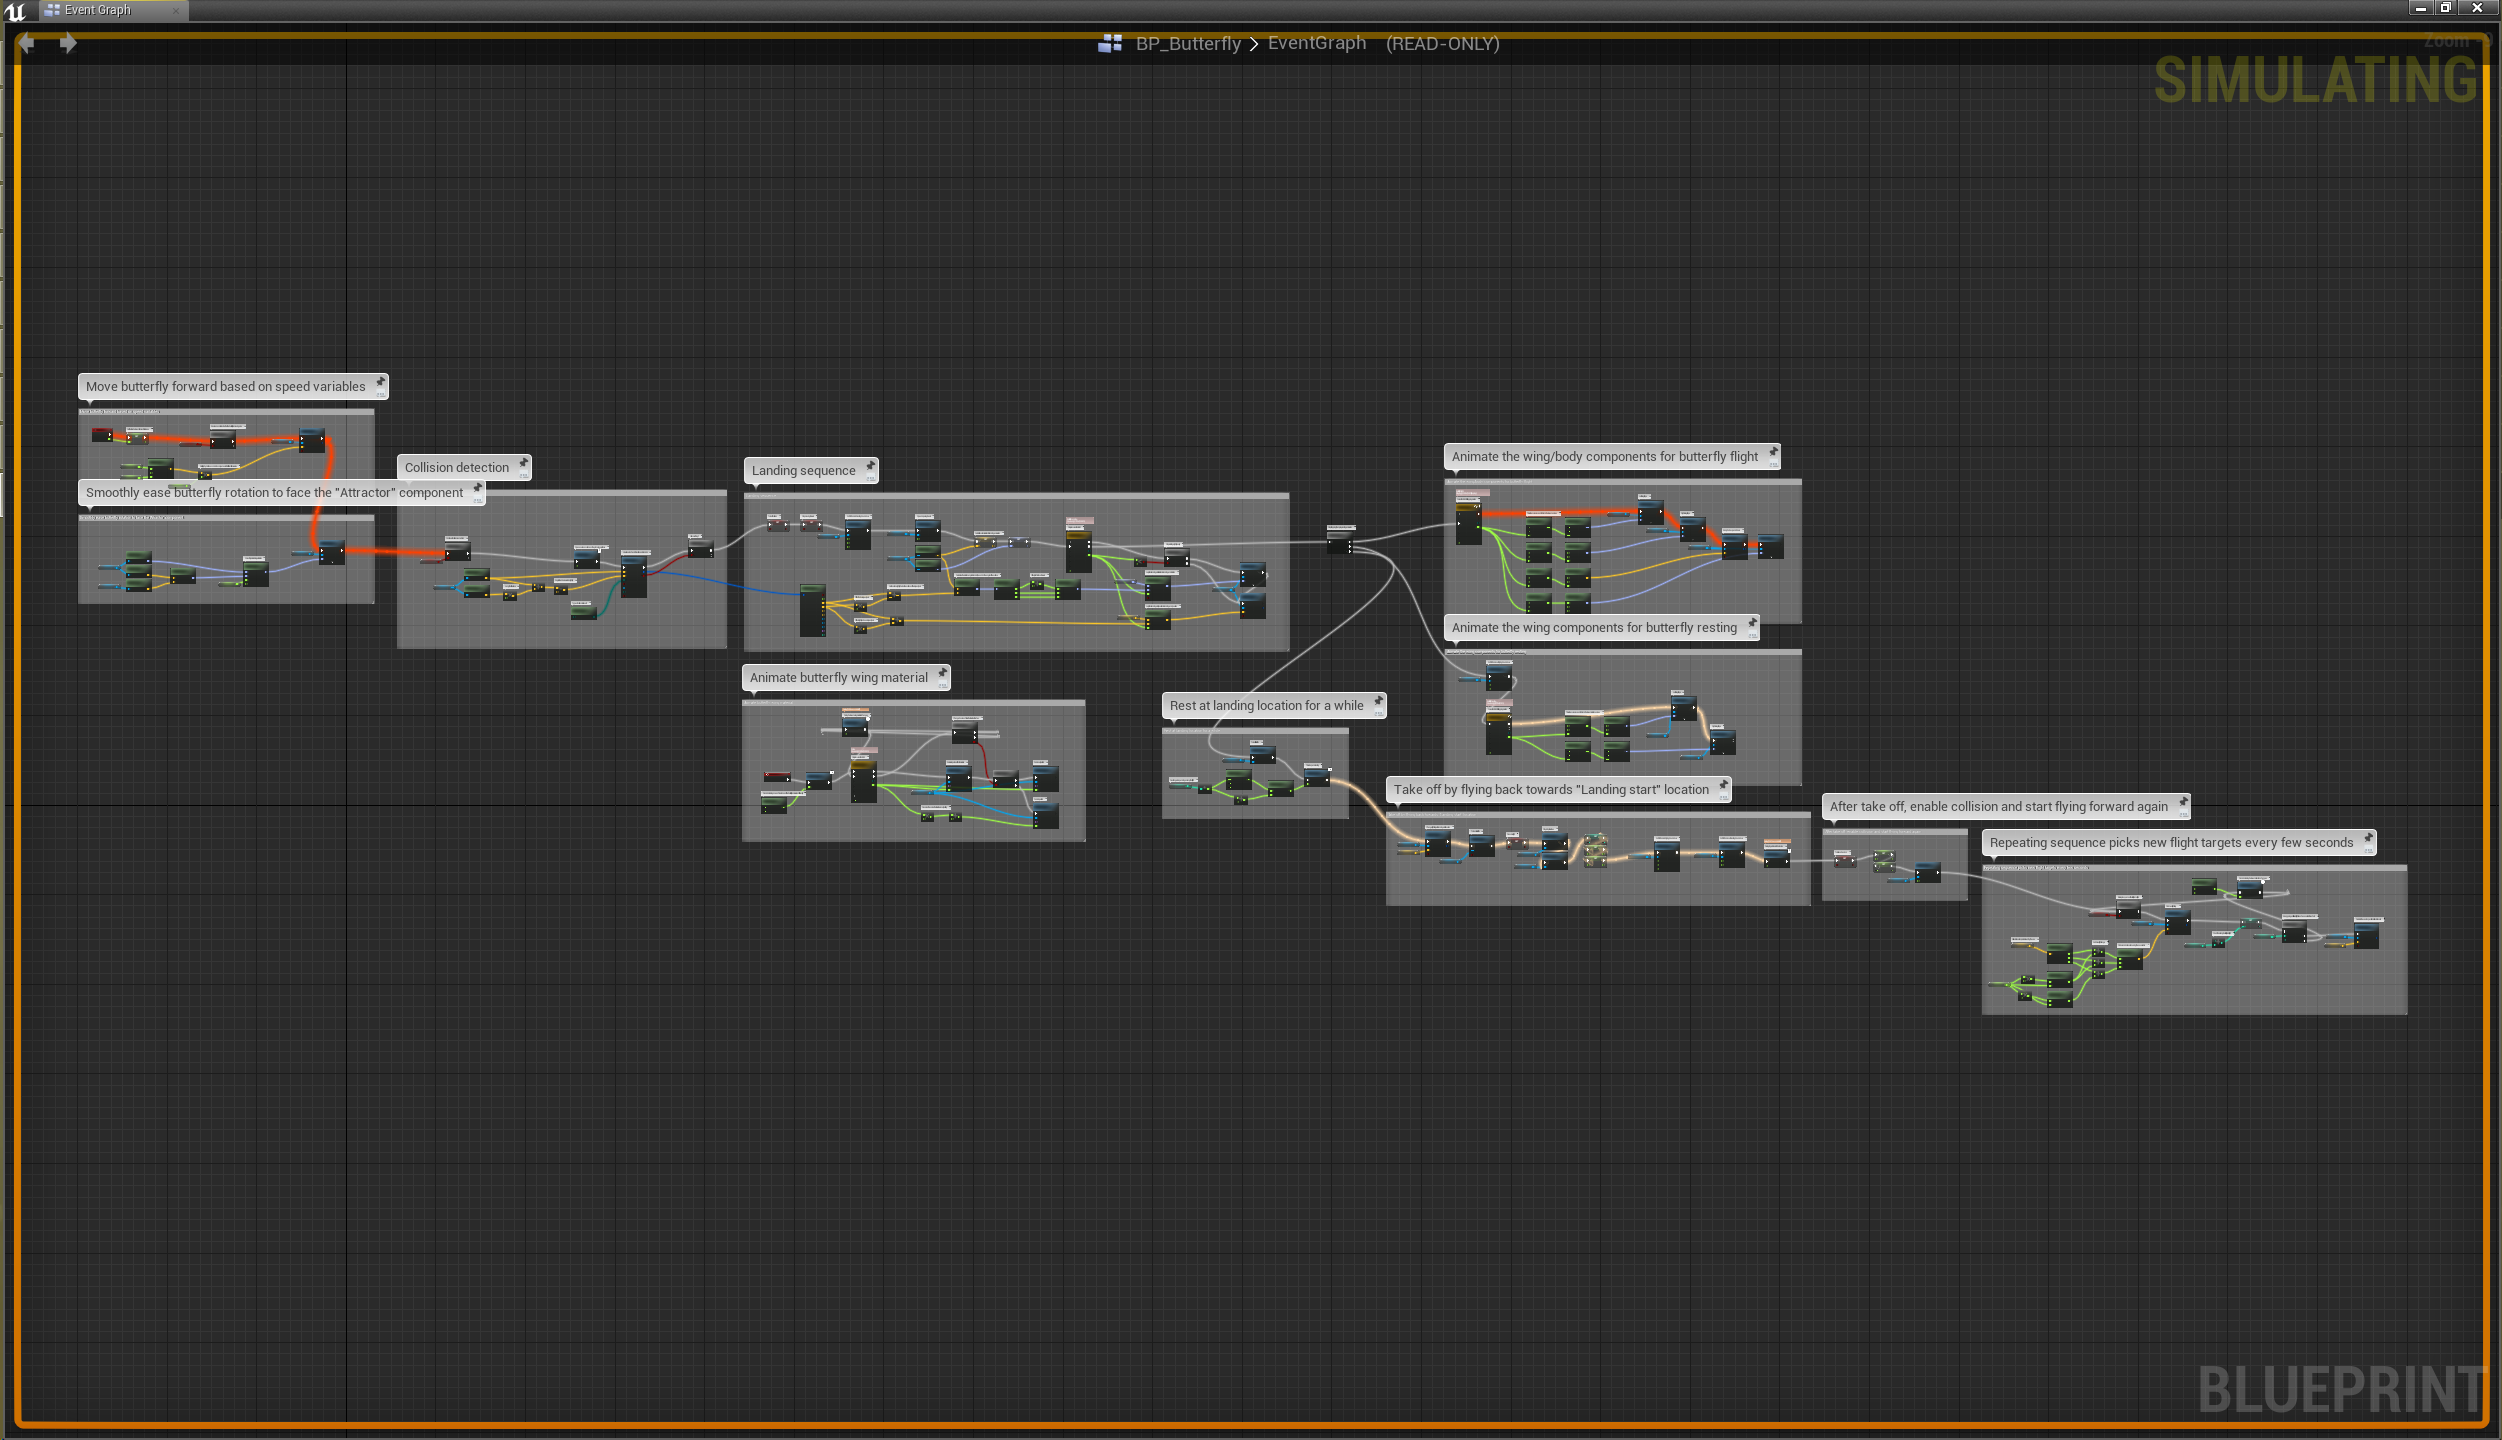
\includegraphics[width=\textwidth]{ue4-blueprint}
% \caption{Unreal Engine 4 Blueprint Beispiel}
% \end{figure}

% http://www.osnews.com/story/19266/WTFs_m
% http://www.gamasutra.com/view/news/239732/Gabe_Newell_shares_how_a_flat_structure_helps_Valve_succeed.php
